\section{Mines and Specifications}

The most common purpose of landmines and unexploded ordnance (UXO) is not necessarily to kill the victim, but to disable personnel and/or equipment. This can result in long-term medical and psychological trauma, as well as being a financial burden for the affected individuals. As well as the mine action, see Figure \ref{fig:contributions_by_thematic_sector_2018}. Areas covered in mines can restrict access to clean water, arable land, roads, healthcare services, and facilities \cite{OxfordAcademic2005}. Therefore, it is easy to see the benefits that can be gained from demining. 

\subsection{What is a landmine}

\begin{wrapfigure}{R}{0.47\linewidth}
\vspace{-8mm}
\centering
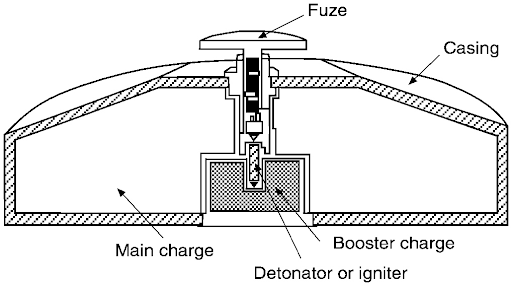
\includegraphics[width=\linewidth]{00 - Images/composition of vehicle landmine.png}
  \caption{Composition of Vehicle Landmine \cite{NAP10071}}
  \label{fig:comp_veh_mine}
\end{wrapfigure}

Landmines are explosive devices with an unmanned trigger mechanism. Landmines are constructed with the specific needs to either disable vehicles or personnel. The content of mines varies based on the target area, but all mines have a trigger mechanism and a main explosive charge. Mines usually consist of an explosive chain reaction being initiated by the trigger mechanism. As in the case with figure \ref{fig:comp_veh_mine} the chronological order of initiation is the fuse then the detonator or ignited followed by the booster charge and finally the main charge. \cite{NAP10071}

\subsection{Mine types}
For landmines to be effective against “enemy” forces they have to be hidden out of sight while close enough for its detonation to release a critical force upon the target/subject. Landmines come in a lot of shapes and sizes ranging from round to square, large and small. The various types of mines have different purposes and can be divided into two main categories being, \gls{ap} mines and \gls{at} mines.


\subsubsection*{\gls{ap} Blast mines} 

\begin{wrapfigure}{R}{0.5\linewidth}
\vspace{-8mm}
\centering
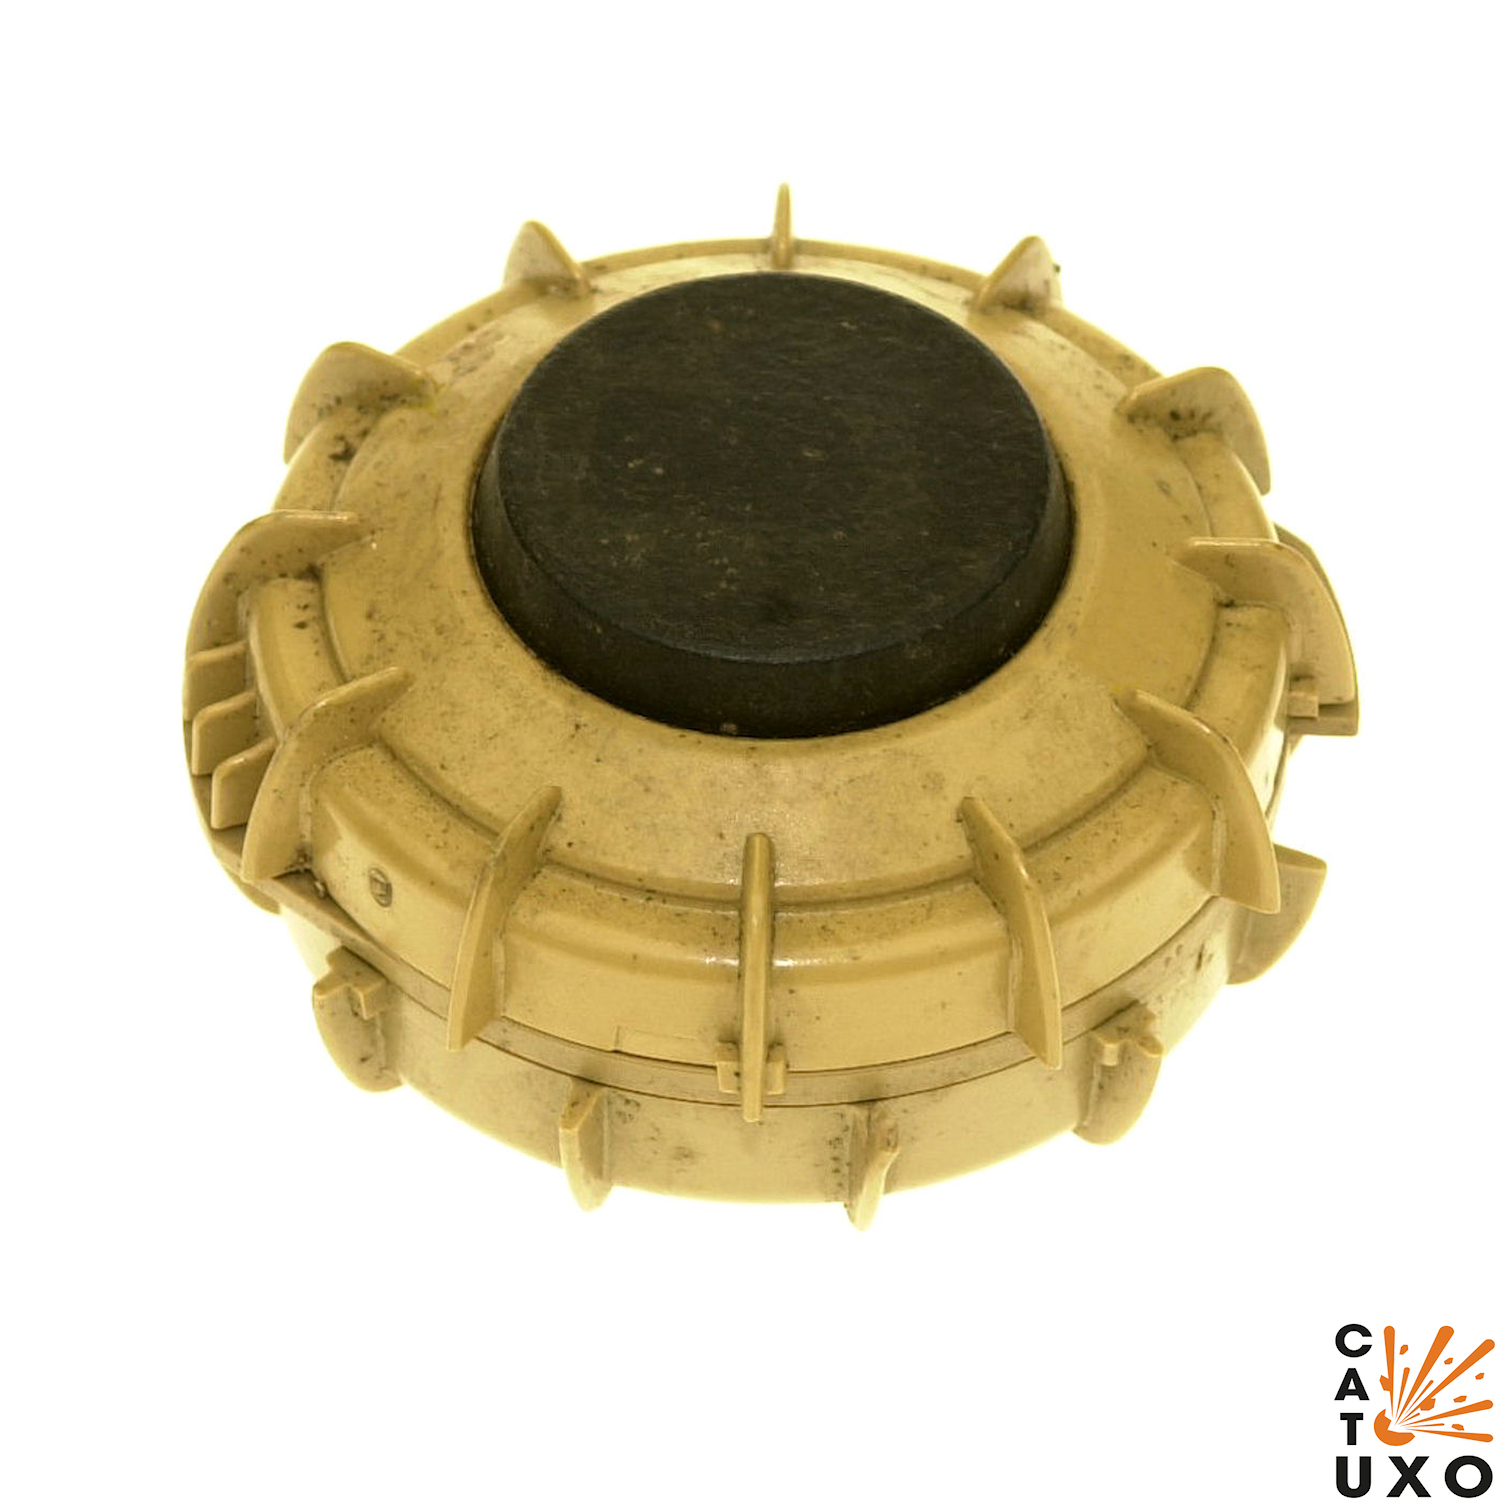
\includegraphics[width=0.5\linewidth]{00 - Images/vs-50-001.jpg}
  \caption{VS-50 Blast mine ø45mm \cite{vs-50}}
  \label{fig:vs-50}
\end{wrapfigure}

These mines are usually placed on the ground or dug into the ground or camouflaged and are designed to detonate when the victim steps on the fuse. Depending on the situation, this mine type does not necessarily kill the victim, instead, it disables the victim. These mines are designed to be small and personnel are the designated targets, thus the diameter ranges from 45-200mm, the operating pressure ranges from 5-16kg and they are usually seen in a circular or rectangular shape \cite{mine_detection}\cite{landmines_and_mine_action}

\newpage

\subsubsection*{\gls{ap} Fragmentation mines}

\paragraph{Bounding}

\begin{wrapfigure}{R}{0.5\linewidth}
\vspace{-8mm}
\centering
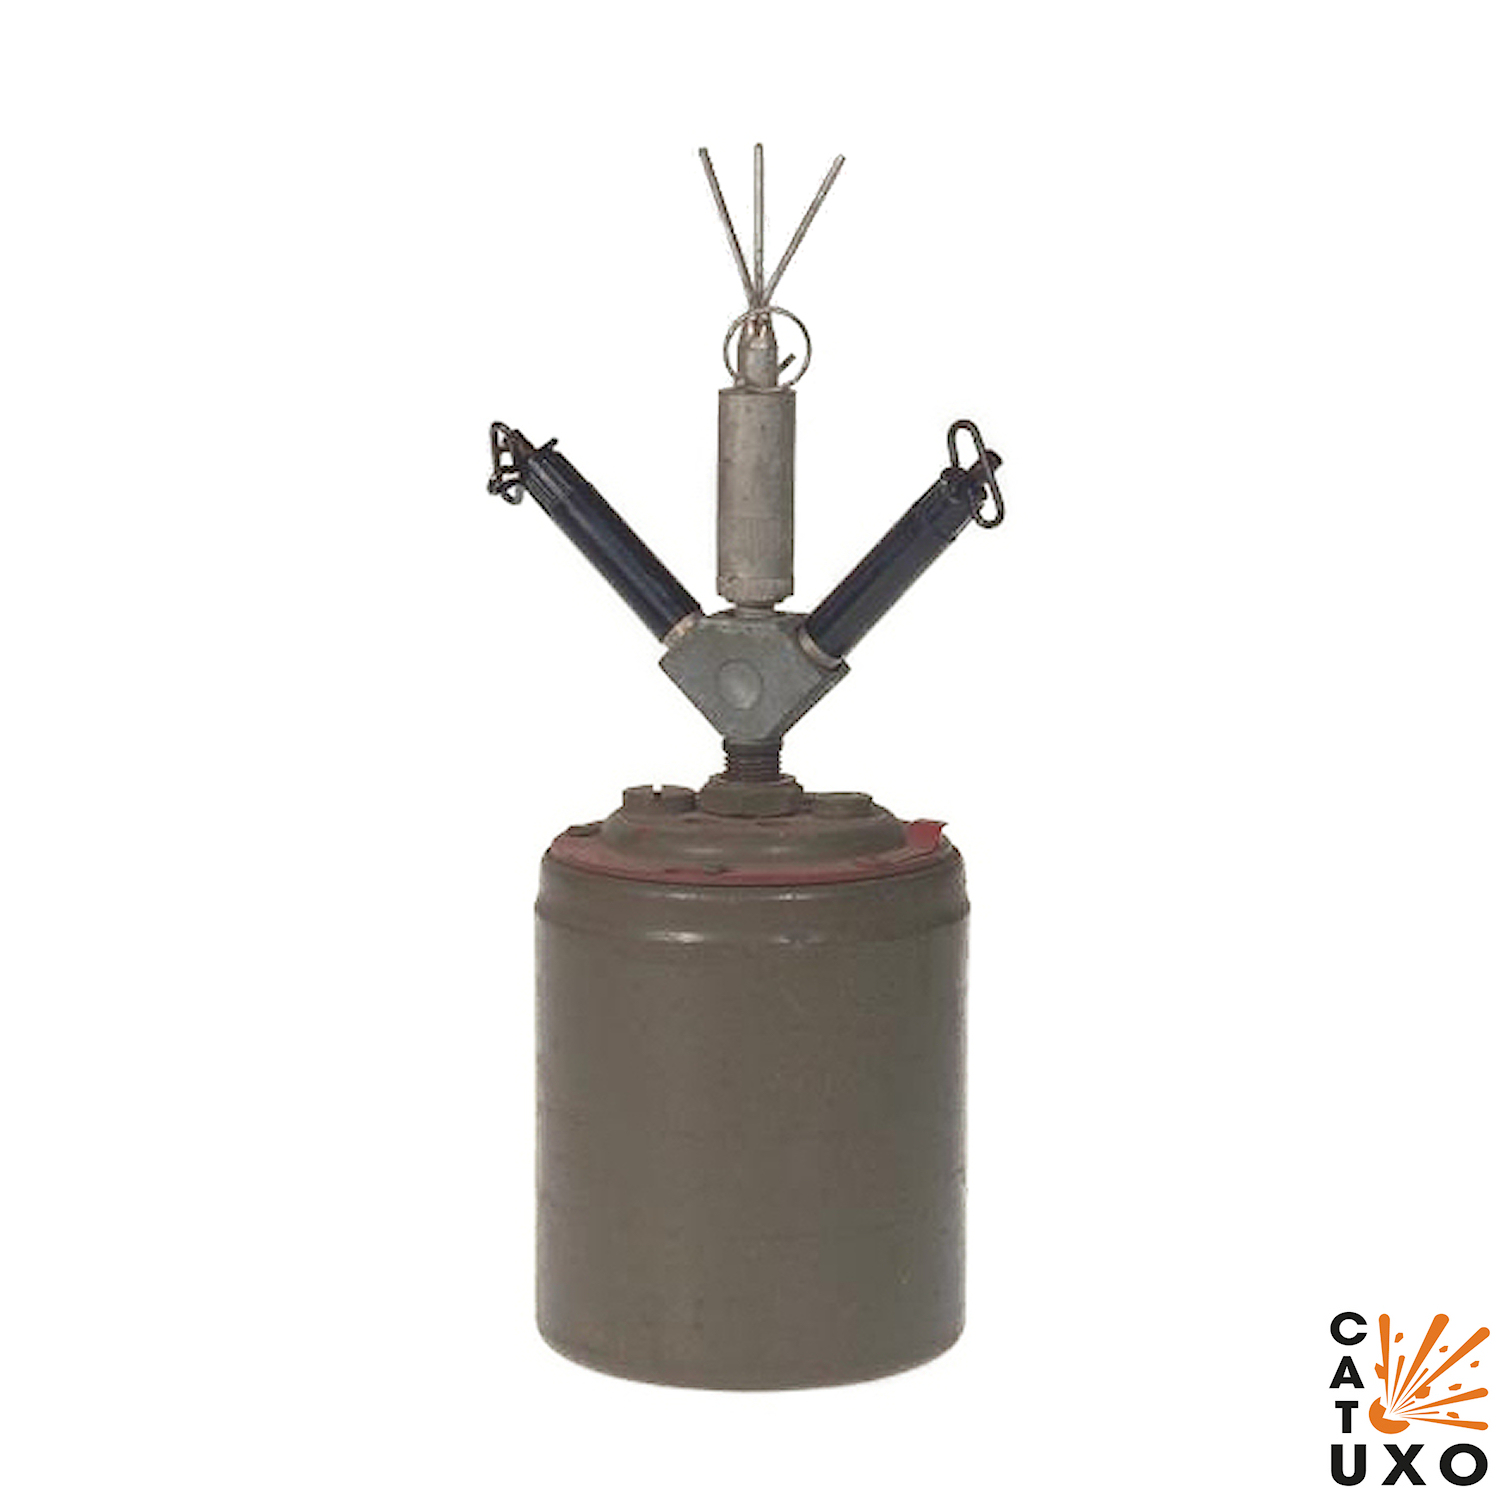
\includegraphics[width=0.5\linewidth]{tex/00 - Images/pp-mi-sr-001.jpg}
  \caption{PP Mi-Sr Bounding mine ø102mm\cite{pp-mi-sr}}
  \label{fig:pp-mi-sr}
\end{wrapfigure}

mines are buried in the ground with the top detonator protruding from the ground and are designed to detonate when a victim comes in contact with the detonator. When activated, the booster charge starts a propellant which lifts the mine approximately 1m into the air, at this point the main charge explodes causing a large amount of damage to the upper part of the body. The specifications of these mines are similar to the \gls{ap} Blast mines, except the height added for the propellant. They are normally found in a cylindrical shape made out of plastic or metal. \cite{mine_detection}


\paragraph{Directional}

\begin{wrapfigure}{R}{0.5\linewidth}
\vspace{-8mm}
\centering
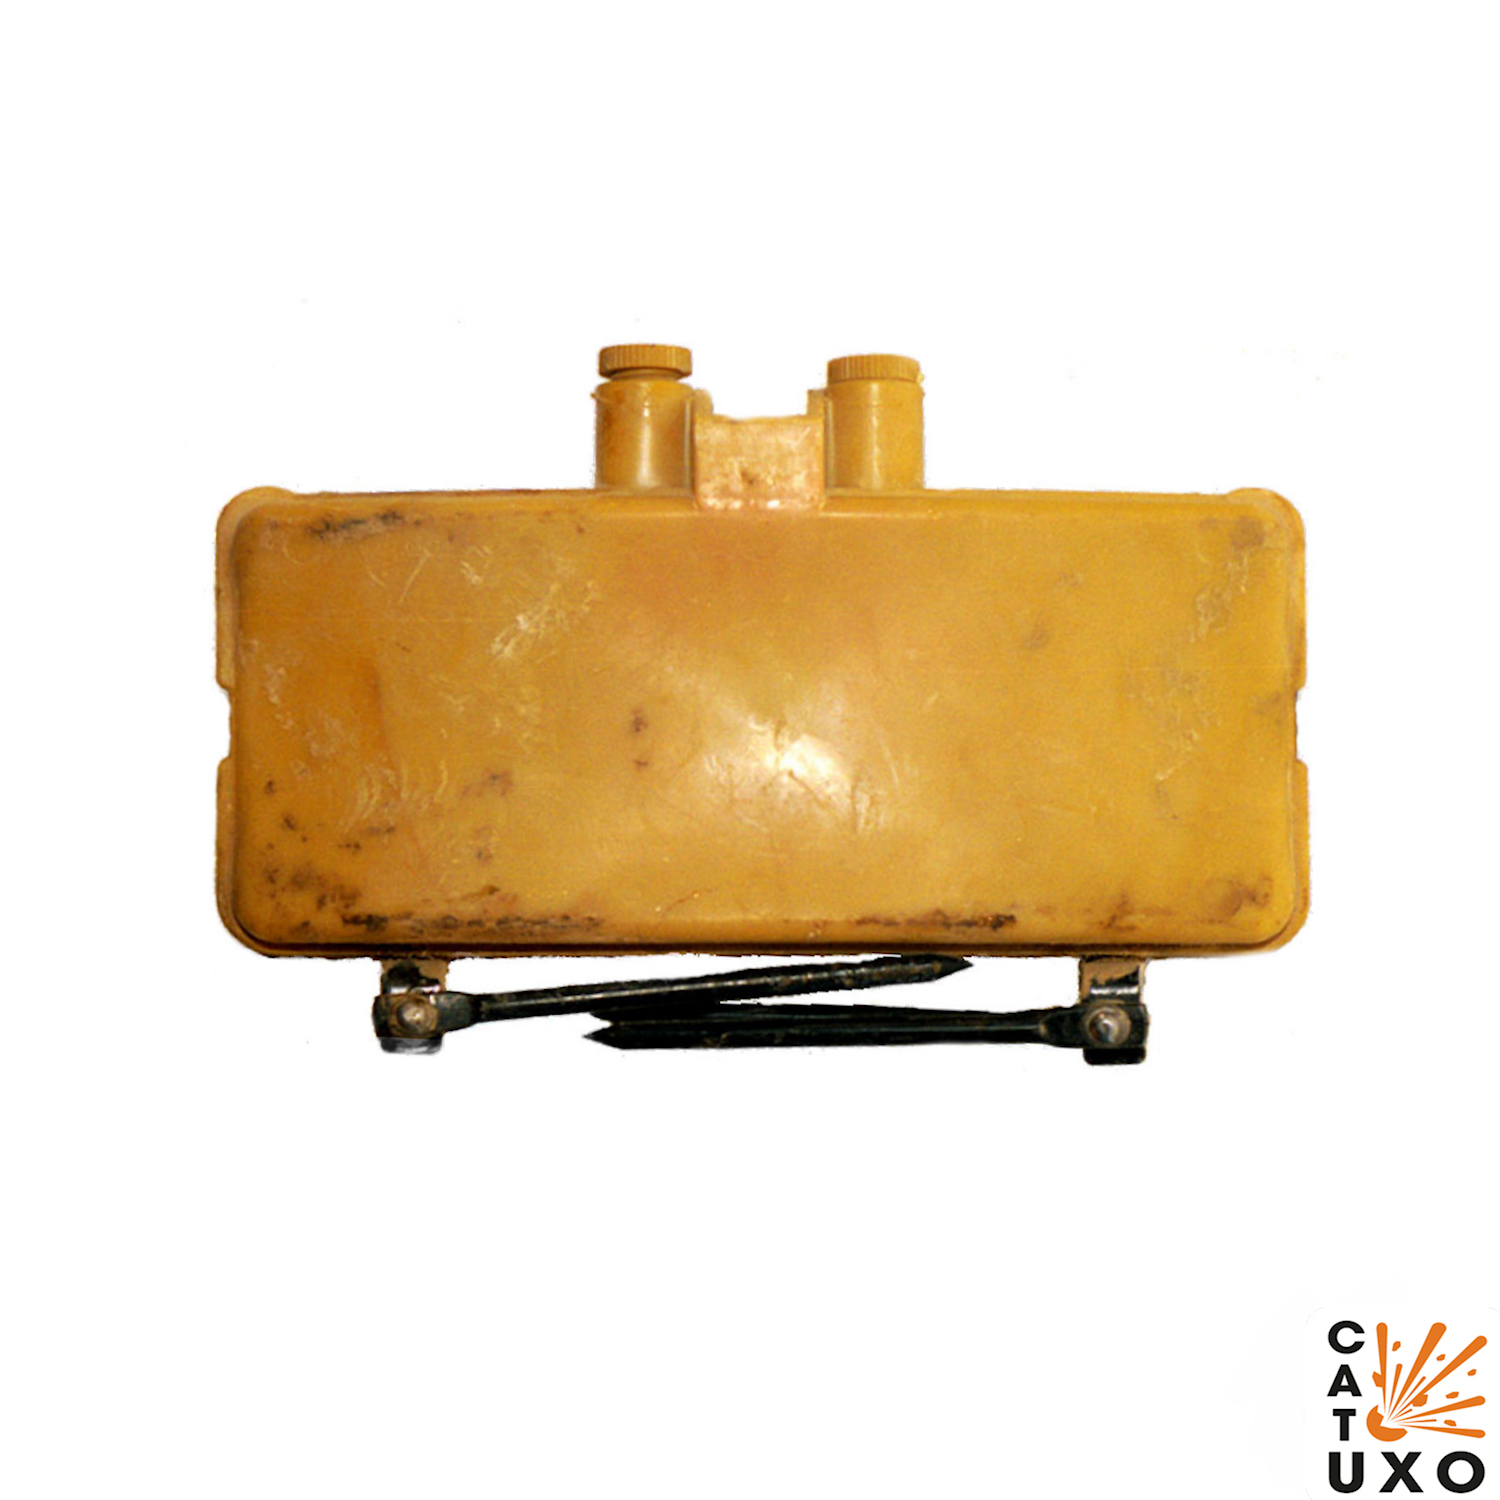
\includegraphics[width=0.5\linewidth]{tex/00 - Images/hamd-y-001.jpg}
  \caption{HAMDY Egyptian Directional mine \cite{hamdy}}
  \label{fig:hamdy}
\end{wrapfigure}

mines are placed on top of the ground supported by their bottom scissor legs, they are usually filled with steel balls or glass, which at detonation fragments in all directions and cause a large amount of injury upon the victim. The directional fragmentation mines are usually triggered by a tripwire or remote detonator and come in rectangular or round shapes made of material such as plastic or metal \cite{mine_detection}


\subsubsection*{\gls{at} mines} 

\begin{wrapfigure}[9]{R}{0.5\linewidth}
\vspace{-8mm}
\centering
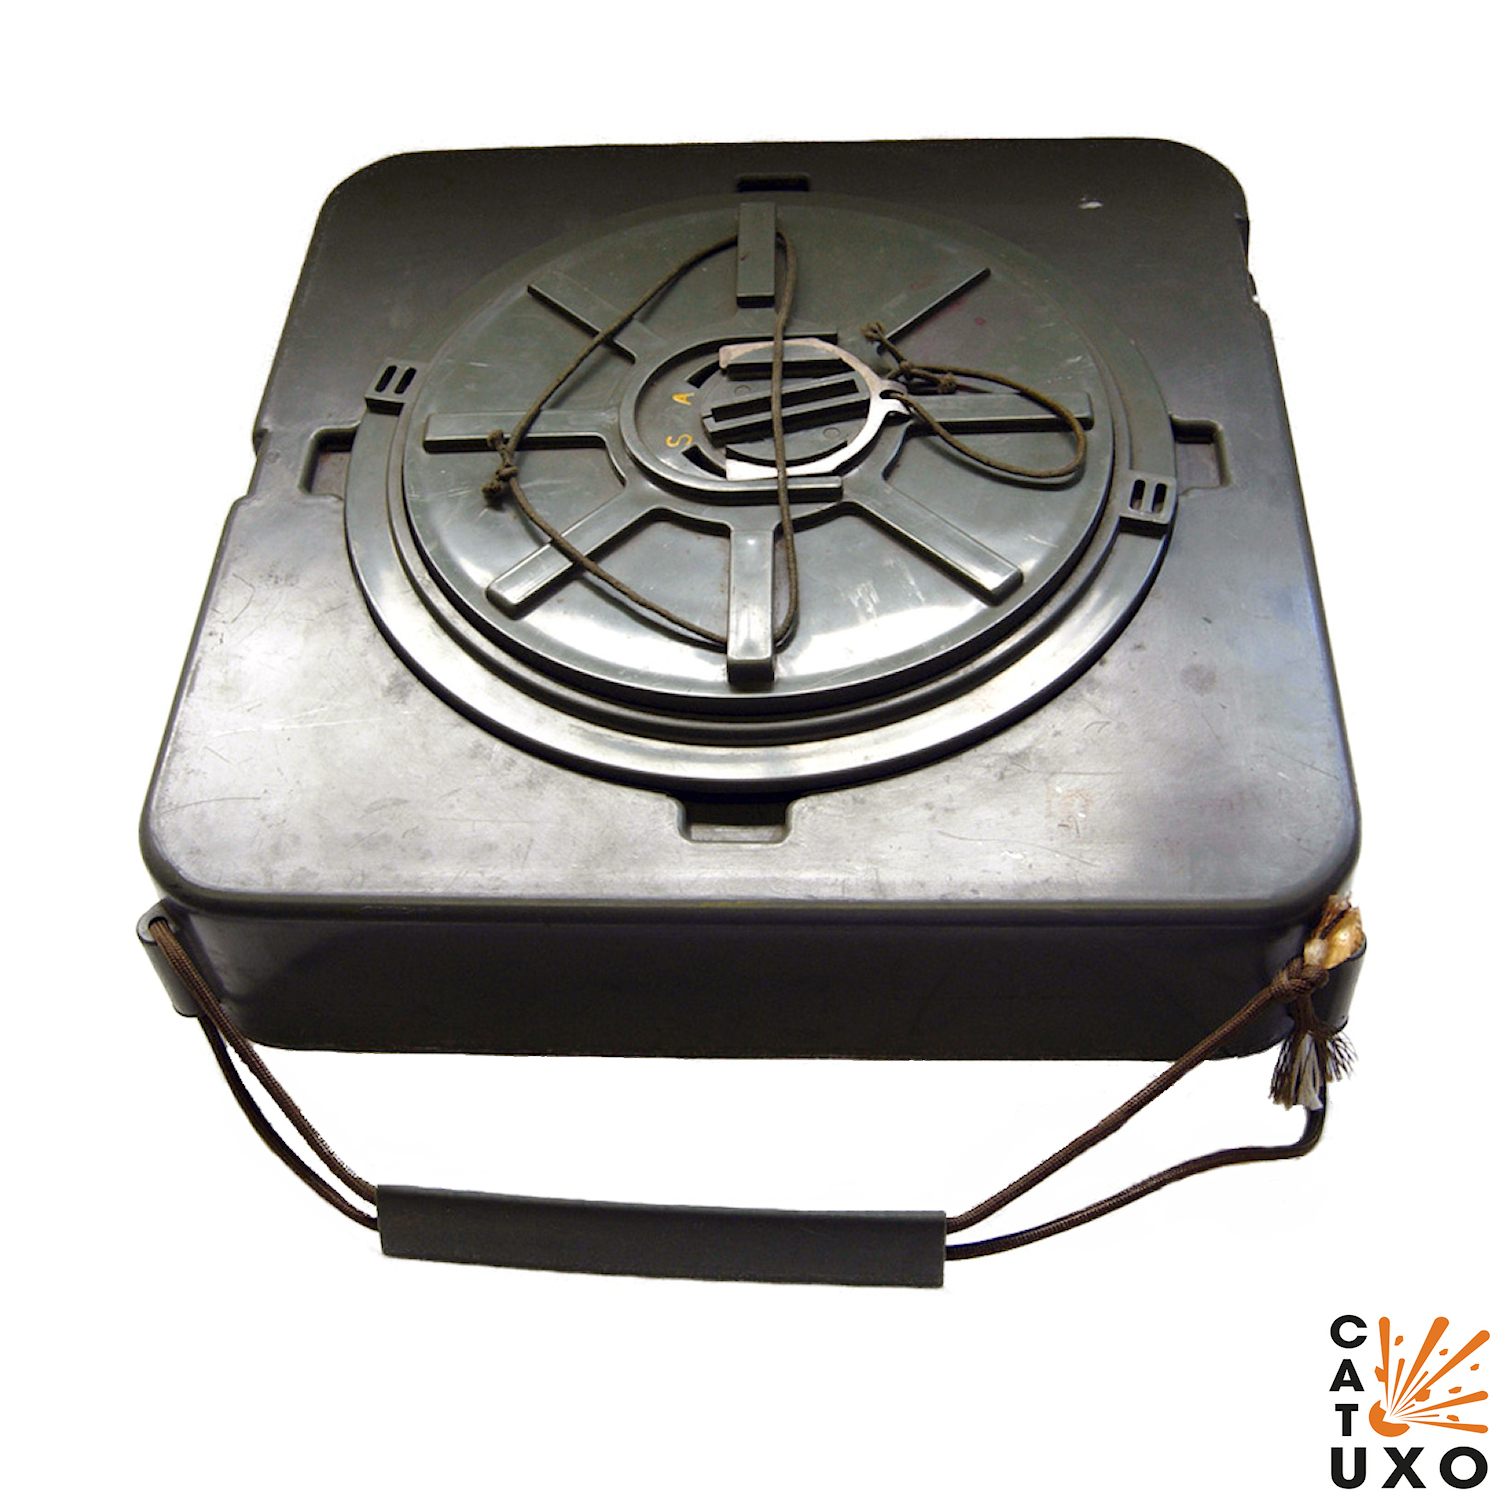
\includegraphics[width=0.5\linewidth]{tex/00 - Images/m19i-003a.jpg}
  \caption{M19 \gls{at} mine \cite{m19}}
  \label{fig:m19}
\end{wrapfigure}

These mines are usually are much larger than the previously mentioned types, due to the fact that they carry a much larger main charge, thus making it able to disable a tank or vehicle, hence the diameter ranges from 45-200mm, the operating pressure is usually 100kg+. Furthermore, these mines are designed in both circular, rectangular, and square shapes in materials such as plastic and metal. \cite{mine_detection}

\subsection{Landmines in Conflict Zones}

For unconventional warfare there are no rules and thereby almost nothing to protect civilians as well as the land from being “affected” more than necessary by the conflict. In this chase it is unlikely that the unconventional force has access to mass production of landmines and therefore makes use of improvised solutions. This could involve re-purposing other types of munition into creative but unorthodox landmines and explosive devices also known as improvised explosive devices (IED).

\newpage

\iffalse
ORIGINAL SEKTION:

Mines are usually simple mechanisms that commonly consist of a container, the internal explosive material, and a trigger. These components can vary according to their intended purpose or accessibility \cite{LandmineDetectionTechniques2010}.


The container can be made with a variety of different materials, ex. plastic, wood, metal, or a combination of those three \cite{LandmineDetectionTechniques2010}. This raises a problem for the mine detection techniques since the materials and size of the explosive device can vary a lot. Improvised mines are usually made with materials available at hand \cite{DetectionAndLocalizationOfImprovisedDevices2010}. That includes both the casing, the explosive material, and the trigger. The trigger component is what will detonate the mine. The mine could be activated by an electronic or pressure sensor. If the mine is intended as an anti-personnel mine with a pressure sensor, then it usually requires a pressure between 5-16 kg to initiate. Anti-tank mines require more than 100kg pressure to initiate. Some mines are buried just below the ground while others have their triggers above the ground \cite{LandmineDetectionTechniques2010}.


The most common purpose of landmines and unexploded ordnance (UXO) is not necessarily to kill the victim, but to disable personnel and/or equipment. This can result in long-term medical and psychological trauma, as well as being a financial burden for the affected individuals. As well as the mine action, see Figure \ref{fig:contributions_by_thematic_sector_2018}. Areas covered in mines can restrict access to clean water, arable land, roads, healthcare services, and facilities \cite{OxfordAcademic2005}. Therefore, it is easy to see the benefits that can be gained from demining. 
\fi

